% !TeX program = pdflatex
\documentclass[12pt,a4paper]{article}
\usepackage{float}


% Русский и базовые настройки
\usepackage[utf8]{inputenc}
\usepackage[T2A]{fontenc}
\usepackage[russian]{babel}
\usepackage{geometry}
\geometry{margin=2.5cm}

% Математика и единицы
\usepackage{amsmath,amssymb,amsthm}
\numberwithin{equation}{section}
\usepackage{siunitx}
\sisetup{locale = DE}


% Графика и ссылки
\usepackage{graphicx}
\usepackage{hyperref}
\usepackage{caption}
\usepackage{booktabs}
\usepackage{enumitem}

% Утилиты
\setlist[itemize]{noitemsep,topsep=2pt}
\setlist[enumerate]{noitemsep,topsep=2pt}

\begin{document}

% ТИТУЛ
\begin{titlepage}
\centering
{\Large Программное обеспечение для определения\\[2pt]
направления магнитных моментов на основе\\[2pt]
магнитооптического эффекта Керра\par}
\vspace{16mm}
\begin{flushleft}
\textbf{Студент:}\\
Моисеев Антон Октаевич\\
группа 419

\vspace{6mm}
\textbf{Руководители:}\\
Перов Николай Сергеевич\\
Голубцов Петр Викторович\\
Перова Наталья Николаевна
\end{flushleft}
\vfill
Москва — 2025
\end{titlepage}

\tableofcontents
\newpage

\section{Введение}

Магнитооптический эффект Керра — изменение поляризации отражённого света от намагниченного материала; наблюдаются вращение плоскости поляризации и эллиптичность, чувствительные к намагниченности в зоне зондирования света. В линейном по намагниченности приближении комплексный керровский угол \(\rho_K=\theta_K+i\epsilon_K\) при p-поляризованном падении аппроксимируется через элементы матрицы отражения как \(\rho_K\approx r_{ps}/r_{pp}\) (для s-падения \(\rho_K\approx r_{sp}/r_{ss}\)); чувствительность определяется внедиагональными компонентами диэлектрического тензора, пропорциональными компонентам \(\mathbf M\).


Магнитооптическая микроскопия по эффекту Керра позволяет визуализировать магнитные домены и их динамику за счёт зависимости поляризационных характеристик отражённого света от вектора намагниченности в зоне зондирования. В тонких плёнках и мультиматериалах эта техника даёт прямую чувствительность к определённой проекции намагниченности, что делает возможным извлечение направления магнитного момента по одиночному или паре изображений. 

Цель работы — разработать и верифицировать алгоритм и программный прототип на Swift/macOS для оценки направления магнитного момента по МОЭК-изображениям с учётом калибровок, устойчивости и метрик качества, а также сформировать целостное описание физической, математической и программной частей.

Данное ПО, разработанное на основе физических законов и классического машинного зрения, не требует серверных мощностей и может быть применимо для анализа различных доменных структур даже на мобильных устройствах, что значительно упрощает и ускоряет анализ различных материалов. 

\section{Магнитооптический эффект Керра (МОЭК) и принципы работы микроскопа Керра}

Магнитооптический эффект Керра (МОЭК), обнаруженный Джоном Керром в 1876 году, является основным явлением, используемым в магнитооптической микроскопии. МОЭК описывает изменение поляризации (вращение $\theta_K$ и эллиптичность $\varepsilon_K$) и/или интенсивности света при его отражении от намагниченной поверхности.

\subsection{Физические основы МОЭК и тензор диэлектрической проницаемости}

Магнитооптические эффекты, такие как МОЭК и вращение Фарадея, имеют свое происхождение в спин-орбитальном и обменном взаимодействиях. В первом порядке эти эффекты линейно зависят от намагниченности $\mathbf{M}$.

\subsubsection{Тензор диэлектрической проницаемости}
МОЭК возникает из-за того, что намагниченность $\mathbf{M}$ делает материал оптически анизотропным. Теория магнитооптики требует рассмотрения тензора диэлектрической проницаемости $\hat{\varepsilon}$, который в присутствии намагниченности принимает недиагональные компоненты. Для изотропных или кубических материалов этот тензор в линейном приближении относительно намагниченности $\mathbf{M} = (m_x, m_y, m_z)$ имеет вид:
$$
\hat{\varepsilon} = \varepsilon_0 \begin{pmatrix} 1 & -i Q m_z & i Q m_y \\ i Q m_z & 1 & -i Q m_x \\ -i Q m_y & i Q m_x & 1 \end{pmatrix}
$$
где $\varepsilon_0$ --- диэлектрическая проницаемость немагнитного материала, а $Q$ --- магнитооптический параметр гирации (или параметр Керра), который является комплексной величиной и определяет силу эффекта.

\subsubsection{Комплексный угол Керра}
Изменение поляризации отражённого света количественно описывается комплексным углом Керра $\Psi_K$, который включает поворот (rotation) $\theta_K$ и эллиптичность (ellipticity) $\varepsilon_K$:
$$
\Psi_K = \theta_K + i\varepsilon_K
$$
Оба этих параметра, $\theta_K$ и $\varepsilon_K$, пропорциональны намагниченности, а также зависят от длины волны света (дисперсии) и оптических констант материала.

\subsubsection{Геометрии МОЭК}
Наблюдаемый эффект зависит от взаимного расположения вектора намагниченности $\mathbf{M}$ и плоскости падения света, что приводит к трём основным геометриям:
\begin{enumerate}
    \item \textbf{Полярный эффект Керра (P-MOKE):} Намагниченность $\mathbf{M}$ перпендикулярна поверхности образца ($m_z \ne 0$). Обычно свет падает нормально или почти нормально.
    \item \textbf{Продольный эффект Керра (L-MOKE):} Намагниченность $\mathbf{M}$ лежит в плоскости образца и параллельна плоскости падения света.
    \item \textbf{Поперечный эффект Керра (T-MOKE):} Намагниченность $\mathbf{M}$ лежит в плоскости образца и перпендикулярна плоскости падения света. T-MOKE уникален тем, что не вызывает вращения поляризации, а приводит к изменению коэффициента отражения (модуляции интенсивности).
\end{enumerate}

\begin{figure}[h]
    \centering
    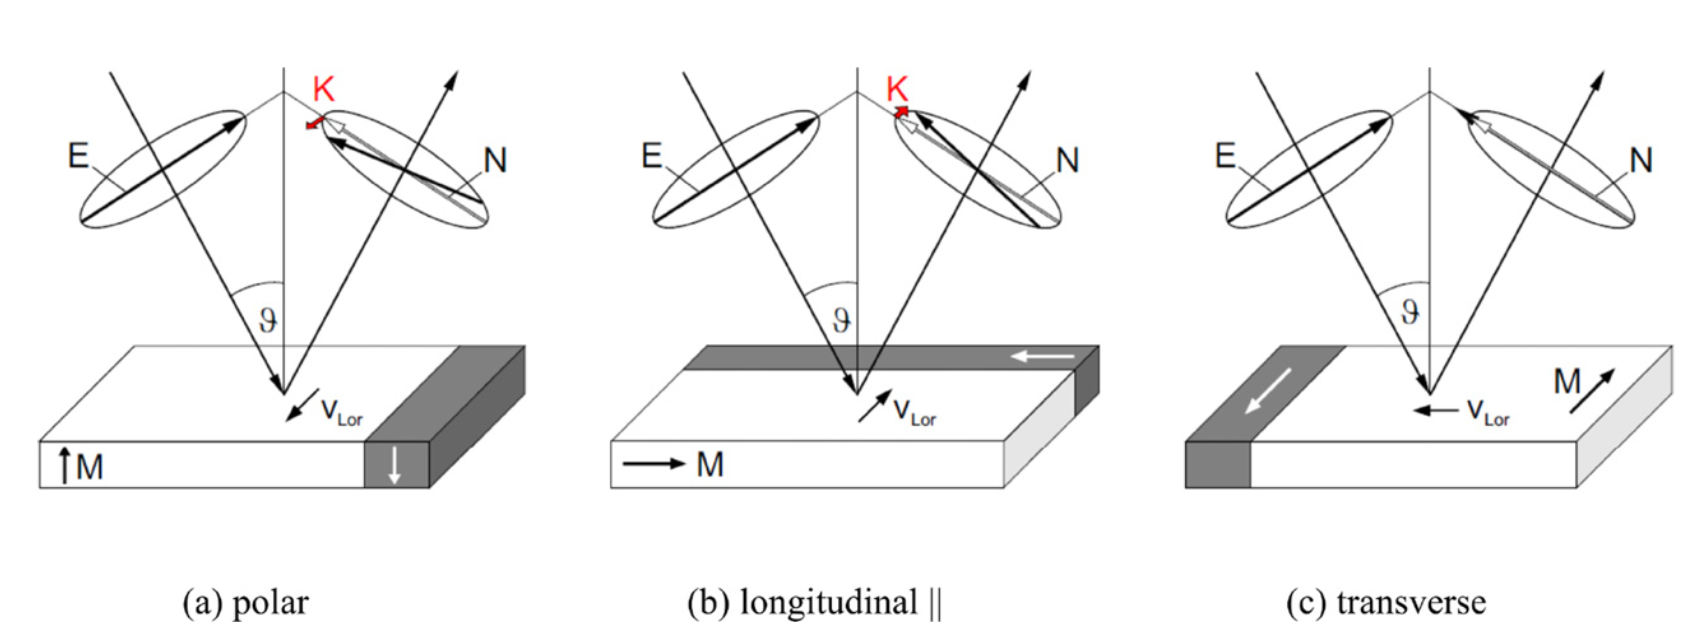
\includegraphics[width=0.8\textwidth]{fig1}
    \caption{Схематическое изображение конфигураций полярного, продольного и поперечного эффектов Керра, иллюстрирующих ориентацию вектора намагниченности $\mathbf{M}$ относительно падающего света.}
\end{figure}

\subsection{Ключевые принципы работы микроскопа Керра и количественный анализ}

МОЭК-микроскопия обычно использует поляризационный оптический микроскоп, где поляризатор создает линейно поляризованный падающий свет, а анализатор преобразует изменение поляризации отраженного света в контраст интенсивности.

\subsubsection{Интенсивность и создание контраста}
В широкопольной (wide-field) микроскопии Керра для создания контраста анализатор устанавливается в положение, близкое к скрещенному (почти гашение света).

Для количественной МОЭК-микроскопии отраженная интенсивность $I$ может быть аппроксимирована как линейная функция компонент намагниченности в плоскости образца:
$$
I = I_0 + Bm_l + Cm_t + D \quad \text{(1)}
$$
где:
\begin{itemize}
    \item $I_0$ — фоновая интенсивность, не зависящая от намагниченности.
    \item $m_l$ и $m_t$ — нормированные продольная и поперечная компоненты намагниченности (вдоль и перпендикулярно плоскости падения).
    \item $B$ и $C$ — коэффициенты, зависящие от нормальных ($N$) и керровских ($K$) амплитуд.
    \item $D$ — член второго порядка по намагниченности (квадратичный), порядка $K^2$.
\end{itemize}
В классическом подходе для наблюдения доменов, не зависящий от намагниченности вклад $I_0$ устраняется с помощью метода разностного изображения. При этом член $D$ (квадратичный по намагниченности) можно пренебречь, если анализатор и поляризатор настроены таким образом, что $N$ велик по сравнению с $K$.

\subsubsection{Векторная и количественная визуализация}
Для полного определения векторного поля намагниченности $\mathbf{M} = (m_x, m_y, m_z)$ в плоскости ($m_x, m_y$) необходимо получить два изображения с ортогональными чувствительностями. В современных микроскопах Керра это достигается путем:
\begin{enumerate}
    \item \textbf{Управления направлением падения:} Используется специальный источник света с массивом из восьми светодиодов, свет которых направляется через оптические волокна. Включение соответствующих светодиодов позволяет устанавливать направление падения света (и, следовательно, направление чувствительности Керра) без механических перемещений. Направление чувствительности (плоскость падения) определяется расположением источника света (концов волокон) в апертурной плоскости объектива.
    \item \textbf{Импульсный режим и вычитание:} Изображения записываются в импульсном режиме с поочередным включением противоположных светодиодов. Вычитание двух изображений, полученных при противоположных направлениях падения света, позволяет получить чистый плоскостной контраст Керра.
    \item \textbf{Устранение паразитного эффекта Фарадея:} Этот импульсный режим с вычитанием также эффективно устраняет паразитные вращения Фарадея, которые возникают в линзе объектива под действием внешнего магнитного поля и искажают сигнал МОЭК.
\end{enumerate}

\subsubsection{Процедура количественной реконструкции}
Количественный анализ требует регистрации двух синусоидальных калибровочных функций, сдвинутых по фазе на $90^\circ$, что обеспечивает два линейных уравнения для двух искомых компонент намагниченности $m_l$ и $m_t$.

В продвинутой методике, разработанной Soldatov и Schäfer, для устранения паразитных вкладов Фарадея и получения чистого контраста, используется разность интенсивностей $I_{\text{diff}}$:
$$
I_{\text{diff}} = I(H) - I(-H)
$$
где $I(H)$ и $I(-H)$ — интенсивности, измеренные при противоположных магнитных полях (или противоположных намагниченных состояниях).

Для реконструкции векторного поля намагниченности $\mathbf{M}$, количественная микроскопия Керра основывается на сравнении интенсивности каждого пикселя, измеренной при двух ортогональных чувствительностях, с локальными калибровочными функциями.

\begin{figure}[h]
    \centering
    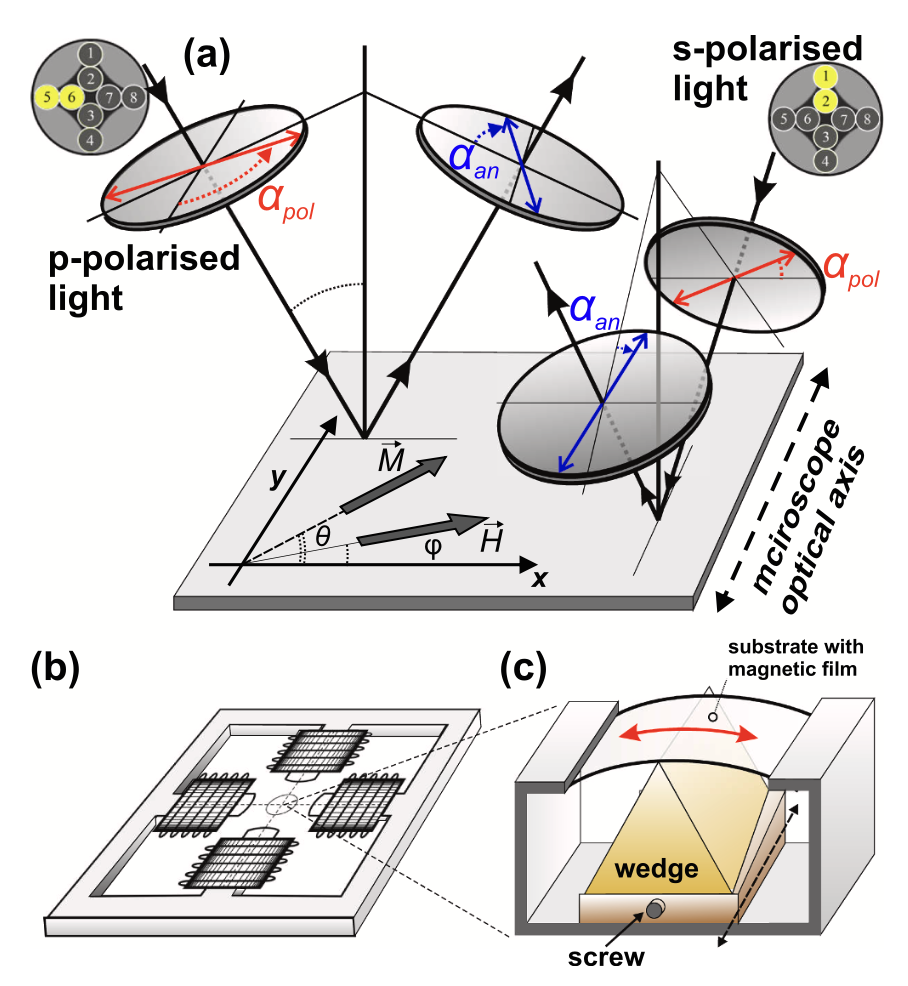
\includegraphics[width=0.8\textwidth]{fig2}
    \caption{Схематическое изображение установки широкопольного МОЭК-магнитометра, включающего массив светодиодов (LED cross), управляемых компьютером, для установки направления падения света и обеспечения ортогональных чувствительностей. (Источник: Рисунок 1(a) из "Advanced, Kerr-microscopy-based MOKE magnetometry for the anisotropy characterisation of magnetic films").}
\end{figure}

\newpage

\section{Постановка задачи}

Физическая часть:
\begin{itemize}
  \item Аналитическое решение задачи.
  \item И тд.
\end{itemize}
Программная часть:
\begin{itemize}
  \item Реализация простого кроссплатформенного UI.
  \item Определения границ доменов с помощью машинного зрения. 
  \item Программное реализация. физических законов.
  \item И тд.
\end{itemize}

\section{Основная часть}

\subsection{Определения границ доменов}

Для анализа изображений магнитных доменов в образцах использовалась разработанная программная реализация метода, основанного на вычислении яркости пикселей и определении светлых и тёмных областей, соответствующих границам доменов.

Анализ начинается с получения матрицы яркости каждого пикселя изображения. Яркость вычисляется по формуле преобразования RGB-компонентов в яркостное значение:

\[
Y = 0.299 \cdot R + 0.587 \cdot G + 0.114 \cdot B
\]

Далее для каждого пикселя проводится классификация на основе пороговых значений яркости, выявляются светлые и тёмные границы доменов. Определяются ключевые точки границ и вычисляются центры доменов, а также векторные поля направлений на основе локальных свойств изображения.

Для визуализации результатов представлены две типовые микроскопические фотографии: исходная (\texttt{figdom1}) и та же фотография с нанесёнными границами доменов (\texttt{figdom2}).

\begin{figure}[H]
    \centering
    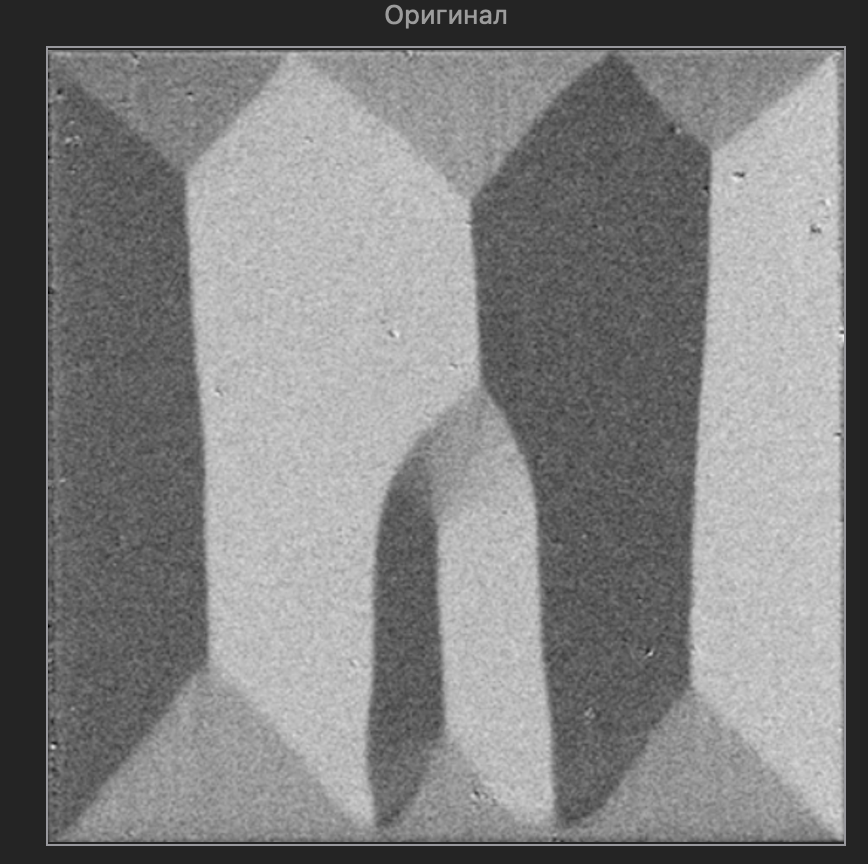
\includegraphics[width=0.8\linewidth]{figdom1}
    \caption{Исходное микроскопическое изображение магнитных доменов.}
    \label{fig:dom1}
\end{figure}

\begin{figure}[H]
    \centering
    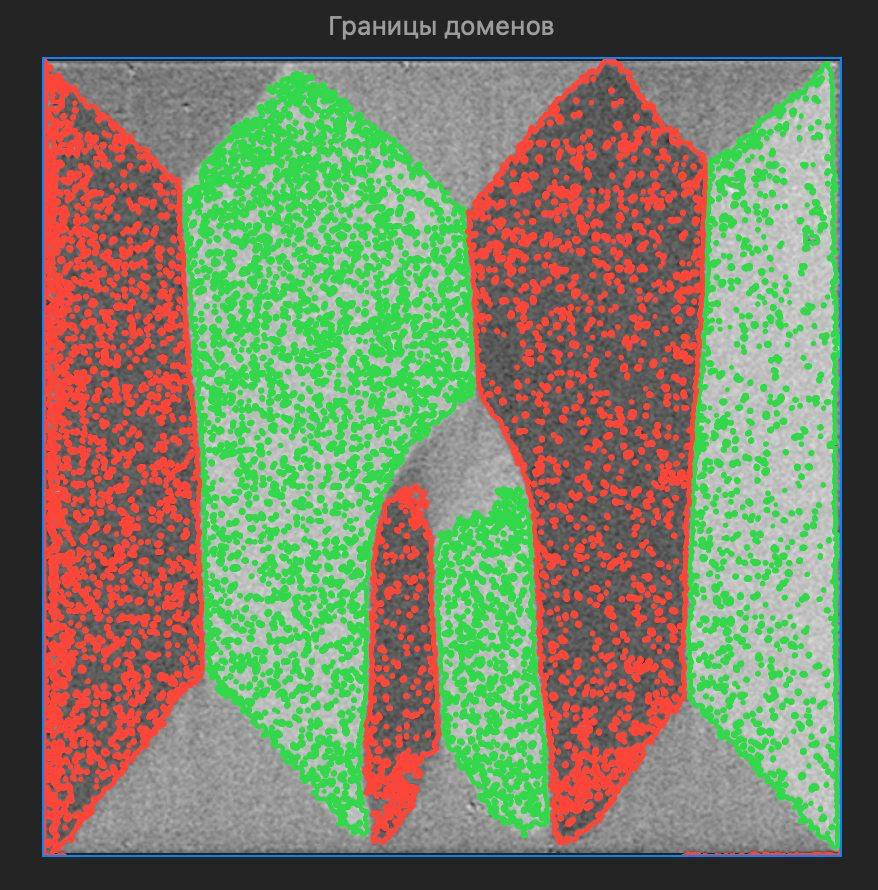
\includegraphics[width=0.8\linewidth]{figdom2}
    \caption{Микроскопическое изображение с наложенными границами доменов, выделенными программным методом.}
    \label{fig:dom2}
\end{figure}

\subsection*{Кратко о физической модели}
МОКЭ проявляется как вращение плоскости поляризации и эллиптичность отражённого света, линейно зависящие (в первом приближении) от соответствующей проекции \(\mathbf M\) на вектор чувствительности \(\mathbf b\), определяемый геометрией (полярной, продольной, поперечной) и оптической настройкой. В режиме «около экстинкции» сигнал фотоинтенсивности становится линейным по \(\rho_K\) и, следовательно, по компоненте \(\mathbf M\), на которую настроена система.

\subsection*{Нормировка и калибровка}
Применяется плоско-полевая коррекция \(I_0(x,y)\) и нормировка \(S=(I-I_0)/I_0\). Для установки абсолютного знака и масштаба выполняется дифференциальная съёмка на насыщении внешнего поля \(+H_{\text{sat}}\) и \(-H_{\text{sat}}\) с построением \(\Delta S\), что фиксирует \(\operatorname{sign}\) и оценивает \(\|\mathbf b\|\) при известной \(M_{\text{sat}}\). В области малого смещения анализатора на угол \(\delta\) от экстинкции интенсивность аппроксимируется
\[
 I_{\text{out}} \approx I_0\left(\delta^2 + 2\,\delta\,\operatorname{Re}\rho_K + |\rho_K|^2\right),
\]
и при \(|\rho_K|\ll \delta \ll 1\) линейная модель по \(\rho_K\) оправдана.

\subsection*{Один кадр и два кадра}
Для одного кадра определяется проекция \(M_{\text{sens}}=(S-a)/\|\mathbf b\|\) и маска доменов с учётом двузначности направления \(\pm\hat{\mathbf b}\). Для пары независимых кадров \(\mathbf b_1,\mathbf b_2\) решается система \(S-a=B\,\mathbf M\) с контролем обусловленности \(\kappa(B)\); при необходимости вводится регуляризация Тихонова.

\subsection*{Подавление шума и карта доверия}
Структурный тензор на изображении используется для оценки локальной когерентности и маскировки доменных стенок (как зон интенсивных градиентов), а также для задания весов уверенности. Визуализация включает векторное поле \(\mathbf M\) и карту доверия, легенду геометрии.

\subsection*{Валидация и метрики}
Используются: угловая ошибка \(\Delta\phi\) на тестовых объёмах и синтетике; метрики сегментации (IoU, F1); стабильность к дрейфу/шуму, проверка линейности при вариации \(\delta\); мониторинг \(\kappa(B)\) и размера регуляризации.

\section{Выводы}
\begin{itemize}
  \item Предложен воспроизводимый конвейер: нормировка → калибровка знака/масштаба → оценка проекции/вектора → маскирование стенок → визуализация и метрики.
  \item Реализуемость на Swift/Core Image/Accelerate подтверждена архитектурой модулей и набором метаданных для повторяемой съёмки и обработки.
  \item Введены критерии устойчивости и качества, позволяющие контролировать применимость линейной модели и корректность восстановления направления \(\mathbf M\).
\end{itemize}

\newpage

\section*{Список литературы} \vspace{-4mm}
\begin{enumerate}
  \item Smith J. Example Article // Some Journal, 2022.
  \item Qiu Z. Q., Bader S. D. Surface magneto-optic Kerr effect // Journal of Magnetism and Magnetic Materials, 2000.
  \item Hubert A., Schäfer R. Magnetic Domains. Springer, 1998.
  \item Zvezdin A. K., Kotov V. A. Modern Magnetooptics and Magnetooptical Materials. Taylor \& Francis, 1997.
  \item Soldatov I. V., Schäfer R. Advanced MOKE magnetometry in wide-field Kerr-microscopy // J. Appl. Phys. 122, 153906 (2017).
  \item Soldatov I. V., Schäfer R. Selective sensitivity in Kerr microscopy // Rev. Sci. Instrum. 88, 073701 (2017).
  \item Soldatov I. V., Schäfer R. Advances in quantitative Kerr microscopy // Phys. Rev. B 95, 014426 (2017).
  \item Schäfer R. Investigation of domains and dynamics of domain walls by the magneto-optical Kerr-effect. In: Handbook of Magnetism and Advanced Magnetic Materials (John Wiley \& Sons, Ltd, 2007).
  \item Kuch W., Schäfer R., Fischer P., Hillebrecht F. Magnetic Microscopy of Layered Structures. Springer, New York, 2015.
  \item Schmidt F., Rave W., Hubert A. Enhancement of magneto-optical Domain observation by digital image-processing // IEEE Trans. Magn. 21, 1596 (1985).
  \item Faraday M. On the magnetisation of light and the illumination of magnetic lines of force // Philos. Trans. R. Soc. London 136, 1 (1846).
  \item Marko D., Soldatov I., Tekielak M., Schäfer R. Stray-field-induced Faraday contributions in wide-field Kerr microscopy and -magnetometry // J. Magn. Magn. Mater. 396, 9 (2015).
  \item Rave W., Reichel P., Brendel H., Leicht M., McCord J., Hubert A. Progress in quantitative magnetic domain observation // IEEE Trans. Magn. 29, 2551 (1993).
  \item Soldatov I., Zehner J., Leistner K., Kang T., Karnaushenko D., Schäfer R. Advanced, Kerr-microscopy-based MOKE magnetometry for the anisotropy characterisation of magnetic films // J. Magn. Magn. Mater. 529, 167889 (2021).
  \item Urs N. O., Mozooni B., Mazalski P., et al. Advanced magneto-optical microscopy: Imaging from picoseconds to centimeters - imaging spin waves and temperature distributions (invited) // AIP Advances 6, 055605 (2016).
  \item Schäfer R., Oppeneer P. M., Ognev A. V., et al. Analyzer-free, intensity-based, wide-field magneto-optical microscopy // Appl. Phys. Rev. 8, 031402 (2021).
  \item Oppeneer P. M. Magneto-optical Kerr spectra. In: Handbook of Magnetic Materials, Vol. 13 (Elsevier, 2001), pp. 229–422.
  \item Rave W., Schäfer R., Hubert A. Quantitative observation of magnetic domains with the magneto-optical Kerr effect // J. Magn. Magn. Mater. 65, 7 (1987).
  \item McCord J., Hubert A. Normalized differential Kerr microscopy an advanced method for magnetic imaging // Phys. Status Solidi A 171, 555–62 (1999).
  \item Wolf G., Hamrle J., Trudel S., et al. Quadratic magneto-optical Kerr effect in Co2MnSi // J. Appl. Phys. 110, 043904 (2011).
  \item Jiménez E., Mikuszeit N., Cuñado J. L. F., et al. Vectorial Kerr magnetometer for simultaneous and quantitative measurements of the in-plane magnetization components // Rev. Sci. Instrum. 85, 053904 (2014).
  \item Teixeira J. M., Lusche R., Ventura J., et al. Versatile, high sensitivity, and automatized angular dependent vectorial Kerr magnetometer for the analysis of nanostructured materials // Rev. Sci. Instrum. 82, 043902 (2011).
  \item Wu T.-h., Fu H., Hajjar R. A., Suzuki T., Mansuripur M. Measurement of magnetic anisotropy constant for magneto-optical recording media: A comparison of several techniques // J. Appl. Phys. 73, 1368–1376 (1993).
  \item Postava K., Jaffres H., Schuhl A., et al. Linear and quadratic magneto-optical measurements of the spin reorientation in epitaxial Fe films on MgO // J. Magn. Magn. Mater. 172, 199–208 (1997).
  \item Kerr J. On rotation of the plane of polarisation by reflection from the pole of a magnet // Philos. Mag. 3, 321–343 (1877).
\end{enumerate}

\newpage
\appendix

\section{Физическое приложение}

\subsection{Магнитные домены и стенки}
Ферромагнитная плёнка разбивается на домены — области квази-единой ориентации \(\mathbf M\), разделённые доменными стенками с быстрым поворотом направления; МОКЭ-микроскопия визуализирует контраст доменов за счёт изменения \(\rho_K\) при смене компоненты \(\mathbf M\), на которую настроена чувствительность.

\subsection{Линейная модель сигнала и ограничения}
Введём нормированный сигнал \(S(x,y)\) после плоско-полевой калибровки:
\begin{equation}
 S(x,y)=\frac{I(x,y)-I_0(x,y)}{I_0(x,y)} \approx a + \mathbf b \cdot \mathbf M(x,y).
\end{equation}
Здесь \(\mathbf b\) — вектор чувствительности, задаваемый геометрией и настройкой поляризатор/анализатор. Одно изображение в фиксированной геометрии определяет лишь проекцию \(\mathbf M\) на \(\mathbf b\) и несёт двузначность \(\pm\) (на \(180^\circ\)) без дополнительной априорной информации (ориентации внешнего поля/калибровки).

\paragraph{Режим около экстинкции и линейность.}
Пусть анализатор смещён от экстинкции на малый угол \(\delta\). Тогда
\begin{equation}
 I_{\text{out}} \approx I_0\Big(\delta^2 + 2\,\delta\,\mathrm{Re}\,\rho_K + |\rho_K|^2\Big),
\end{equation}
и для \(|\rho_K| \ll \delta \ll 1\) вклад \(2\delta\,\mathrm{Re}\,\rho_K\) доминирует, обосновывая линейную аппроксимацию \(S\simeq a+\mathbf b\cdot\mathbf M\). Практически следует контролировать \(\delta\) в эксперименте и проверять линейность по серии малых \(\delta\).

\section{Математическое приложение}
\subsection{Постановка}
По входному МОКЭ-изображению \(I(x,y)\) и метаданным съёмки восстановить: при одном кадре — карту возможных направлений \(\pm\hat{\mathbf b}\) и знак проекции \(M_{\text{sens}}\); при двух независимых кадрах — вектор \((M_x,M_y)\) в плоскости образца.

\subsection{Нормировка и наблюдаемые}
Оценивается плоское поле \(I_0(x,y)\) и определяется
\begin{equation}
 S(x,y)=\frac{I(x,y)-I_0(x,y)}{I_0(x,y)}.
\end{equation}
Геометрия съёмки задаёт единичный \(\hat{\mathbf b}\) и масштаб \(\|\mathbf b\|\).

\subsection{Линейная модель и один кадр}
При фиксированной геометрии
\begin{equation}
 S(x,y)=a+\mathbf b\cdot \mathbf M(x,y).
\end{equation}
Оценка «чувствительной» проекции:
\begin{equation}
 M_{\text{sens}}(x,y)=\frac{S(x,y)-a}{\|\mathbf b\|}, \qquad \text{направление: } \pm \hat{\mathbf b}.
\end{equation}
Выводится карта знака и величины проекции с учётом двузначности.

\subsection{Два независимых кадра}
Для двух кадров с линейно независимыми \(\mathbf b_1,\mathbf b_2\) (в плоскости образца):
\begin{equation}
 \begin{bmatrix} S_1-a_1\\ S_2-a_2 \end{bmatrix}
 =
 \underbrace{\begin{bmatrix} b_{1x} & b_{1y}\\ b_{2x} & b_{2y}\end{bmatrix}}_{B}
 \begin{bmatrix} M_x\\ M_y \end{bmatrix}.
\end{equation}
Тогда \(\,(M_x,M_y)^\top = B^{-1}(S-a)\,\) при \(\det B\neq 0\). Для улучшения устойчивости при большой \(\kappa(B)\) используется
\begin{equation}
 \mathbf M = (B^\top B + \lambda I)^{-1}B^\top (S-a),
\end{equation}
где \(\lambda>0\) — малая регуляризация.

\subsection{Сегментация доменов}
Трёхзначная маска:
\begin{equation}
 D(x,y)=
 \begin{cases}
 +1, & M_{\text{sens}} > T,\\
 -1, & M_{\text{sens}} < -T,\\
 0, & |M_{\text{sens}}|\le T,
 \end{cases}
\end{equation}
где \(T\) — робастный порог (например, по MAD) после сглаживания и вычитания фона.

\subsection{Оценка локальной ориентации: структурный тензор}
Пусть \(I_x,I_y\) — градиенты. Структурный тензор
\begin{equation}
 J = G_\rho * 
 \begin{bmatrix}
 I_x^2 & I_x I_y\\
 I_x I_y & I_y^2
 \end{bmatrix}.
\end{equation}
Угол локальной ориентации
\begin{equation}
 \phi = \tfrac12 \arctan2\!\big(2J_{xy},\, J_{xx}-J_{yy}\big),
\end{equation}
когерентность 
\begin{equation}
 c=\frac{\lambda_1-\lambda_2}{\lambda_1+\lambda_2},
\end{equation}
где \(\lambda_1\ge\lambda_2\) — собственные значения \(J\). Значение \(c\) используется для подавления шумовых областей и маскировки доменных стенок.

\subsection{Предобработка и устойчивость}
Применяются: гауссово сглаживание \(G_\sigma * I\), вычитание медленного фона, морфологические операции (open/close), адаптивный порог; доверие пикселя по \(|S|\) и \(c\). Эти шаги стабилизируют знак и границы доменов перед визуализацией.

\subsection{Калибровка на насыщении и знак}
Снимается пара кадров при \(+H_{\text{sat}}\) и \(-H_{\text{sat}}\) в неизменной геометрии:
\begin{equation}
 \Delta S = S(+H_{\text{sat}})-S(-H_{\text{sat}}) \approx 2\,\|\mathbf b\|\,M_{\text{sat}}\cdot \operatorname{sign}.
\end{equation}
Это задаёт абсолютный знак и позволяет оценить \(\|\mathbf b\|\) при известном \(M_{\text{sat}}\). Рекомендуется сохранять \(\Delta S\) как эталон для серии.

\subsection{Проверка независимости и ковариация}
Линейная независимость \(\mathbf b_1,\mathbf b_2\) контролируется по \(|\det B|\) и \(\kappa(B)\). При гауссовском шуме с ковариацией \(\Sigma\) ковариация оценки
\begin{equation}
 \mathrm{Cov}(\mathbf M) \approx (B^\top \Sigma^{-1} B)^{-1}.
\end{equation}
Это используется для построения карты доверия и отбора пикселей.

\subsection{Псевдокод конвейера}
\begin{enumerate}
  \item Стабилизация и flat-field: оценить \(I_0\), получить \(S=(I-I_0)/I_0\).
  \item Калибровка: снять \(\Delta S\) на \(\pm H_{\text{sat}}\), установить знак и \(\|\mathbf b\|\).
  \item Один кадр: \(M_{\text{sens}}=(S-a)/\|\mathbf b\|\), пороговая маска после сглаживания.
  \item Два кадра: собрать \(S_1,S_2\), проверить \(\kappa(B)\), восстановить \(\mathbf M\) с регуляризацией при необходимости.
  \item Структурный тензор: посчитать \(c\), замаскировать стенки и шумовые зоны.
  \item Визуализация: карта знака/вектора, карта доверия, легенда геометрии.
\end{enumerate}

\section{Программное приложение}

В рамках работы было разработано настольное приложение на языке Swift для macOS с использованием фреймворка SwiftUI. Цель приложения — предоставить удобный инструмент для загрузки МОЭК-изображений, автоматического выделения доменных областей и границ доменов, а также визуализации векторного поля, соответствующего локальному направлению магнитного момента. Приложение реализует описанный ранее алгоритм обработки изображений и позволяет наглядно сравнивать исходные данные с результатами анализа.

\subsection{Общая архитектура}

Приложение состоит из трёх основных модулей:

\begin{itemize}
    \item \textbf{course4\_programApp.swift} — точка входа в приложение, задающая корневое окно и подключающая основной интерфейс.
    \item \textbf{ContentView.swift} — пользовательский интерфейс на SwiftUI, обеспечивающий загрузку изображения, запуск анализа и отображение результатов.
    \item \textbf{generateVectorDiagram.swift} — модуль алгоритмов обработки изображения, включающий вычисление яркости, определение доменных областей и границ, построение векторного поля и подготовку данных для визуализации.
\end{itemize}

Общая схема работы такова: пользователь выбирает изображение, интерфейс передаёт его в модуль анализа, который возвращает структуру данных с векторами и набором ключевых точек. Затем эти данные отображаются поверх исходного изображения в виде стрелок и линий границ доменов.

\subsection{Точка входа: \texttt{course4\_programApp.swift}}

Этот файл задаёт основное окно приложения и подключает корневое представление интерфейса:

\begin{verbatim}
import SwiftUI

@main
struct course4_programApp: App {
    var body: some Scene {
        WindowGroup {
            ContentView()
        }
    }
}
\end{verbatim}

Аннотация \texttt{@main} помечает структуру как точку входа. Внутри \texttt{body} создаётся сцена \texttt{WindowGroup}, в которой в качестве корневого представления используется \texttt{ContentView}. Таким образом, при запуске приложения автоматически открывается окно с основным интерфейсом анализа доменов.

\subsection{Пользовательский интерфейс: \texttt{ContentView.swift}}

Файл \texttt{ContentView.swift} реализует основное окно приложения, включая загрузку изображения, запуск анализа и отображение результатов. Упрощённая структура файла выглядит следующим образом:

\begin{verbatim}
import SwiftUI
import UniformTypeIdentifiers
import AppKit

struct ContentView: View {
    @State private var image: NSImage?
    @State private var vectorArrows: [Arrow] = []
    @State private var brightBoundaryPoints: [CGPoint] = []
    @State private var darkBoundaryPoints: [CGPoint] = []
    @State private var showVectorDiagram: Bool = false

    private let canvasSize: CGFloat = 400

    var body: some View {
        VStack(spacing: 16) {
            controlsSection
            Divider()
            ScrollView {
                if let nsImage = image {
                    imageAndResultsView(nsImage: nsImage)
                } else {
                    Text("Загрузите изображение для анализа")
                }
            }
            .padding()
        }
        .frame(minWidth: 600, minHeight: 500)
    }
}
\end{verbatim}

Здесь хранятся несколько \texttt{@State}-переменных: загруженное изображение \texttt{image}, массив стрелок \texttt{vectorArrows}, списки точек светлых и тёмных границ доменов (\texttt{brightBoundaryPoints}, \texttt{darkBoundaryPoints}) и флаг \texttt{showVectorDiagram}, отвечающий за отображение векторной диаграммы поверх изображения.

Блок \texttt{controlsSection} содержит кнопки для загрузки файла и запуска анализа. Типичный код выглядит так:

\begin{verbatim}
private var controlsSection: some View {
    HStack(spacing: 12) {
        Button("Открыть изображение") {
            openImageFile { selectedImage in
                self.image = selectedImage
                self.vectorArrows = []
                self.brightBoundaryPoints = []
                self.darkBoundaryPoints = []
                self.showVectorDiagram = false
            }
        }

        Button("Анализировать домены") {
            if let img = image {
                let vis = analyzeDomains(from: img,
                                         targetSize: canvasSize)
                self.vectorArrows = vis.arrows
                self.brightBoundaryPoints = vis.brightBoundaryPoints
                self.darkBoundaryPoints = vis.darkBoundaryPoints
                self.showVectorDiagram = true
            }
        }
        .disabled(image == nil)
    }
    .padding(.top, 16)
}
\end{verbatim}

Функция \texttt{openImageFile} открывает системное диалоговое окно выбора файла (через \texttt{NSOpenPanel}), считывает выбранное изображение и передаёт его в обработчик. Кнопка «Анализировать домены» вызывает функцию \texttt{analyzeDomains(from:targetSize:)} из модуля обработки, которая возвращает структуру с результатами анализа (стрелки и точки границ доменов).

Отображение изображения и результатов реализовано через связку \texttt{Image} и \texttt{Canvas}. Сначала показывается исходное изображение, а при включённом флаге \texttt{showVectorDiagram} поверх него рисуются стрелки и точки границ:

\begin{verbatim}
private func imageAndResultsView(nsImage: NSImage) -> some View {
    VStack(spacing: 24) {
        VStack(spacing: 8) {
            Text("Исходное изображение")
                .foregroundColor(.secondary)
            Image(nsImage: nsImage)
                .resizable()
                .scaledToFit()
                .frame(width: canvasSize, height: canvasSize)
        }

        if showVectorDiagram {
            VStack(spacing: 8) {
                Text("Векторная диаграмма и границы доменов")
                    .foregroundColor(.secondary)

                Canvas { context, size in
                    drawVectorDiagram(in: context, size: size)
                }
                .frame(width: canvasSize, height: canvasSize)
            }
        }
    }
}
\end{verbatim}

Функция \texttt{drawVectorDiagram} отрисовывает:

\begin{itemize}
    \item стрелки векторов намагниченности из массива \texttt{vectorArrows};
    \item точки (или маркеры) светлых границ доменов (\texttt{brightBoundaryPoints});
    \item точки тёмных границ доменов (\texttt{darkBoundaryPoints}), которые можно выделять другим цветом.
\end{itemize}

Таким образом, \texttt{ContentView.swift} отвечает за взаимодействие с пользователем и визуализацию, а основная математика и анализ спрятаны в отдельном модуле.

\subsection{Алгоритмы анализа: \texttt{generateVectorDiagram.swift}}

Файл \texttt{generateVectorDiagram.swift} содержит реализацию вычислительной части. В нём определена структура \texttt{DomainVisualization}, описывающая результат анализа, и функция \texttt{analyzeDomains(from:targetSize:)}, которая и вызывается из интерфейса.

\begin{verbatim}
import SwiftUI
import AppKit

struct Arrow {
    let start: CGPoint
    let end: CGPoint
}

struct DomainVisualization {
    let arrows: [Arrow]
    let brightBoundaryPoints: [CGPoint]
    let darkBoundaryPoints: [CGPoint]
}

func analyzeDomains(from image: NSImage,
                    targetSize: CGFloat = 400) -> DomainVisualization {
    // 1. Получение растрового представления
    guard let tiffData = image.tiffRepresentation,
          let bitmap = NSBitmapImageRep( tiffData) else {
        return DomainVisualization(arrows: [],
                                   brightBoundaryPoints: [],
                                   darkBoundaryPoints: [])
    }

    let width = bitmap.pixelsWide
    let height = bitmap.pixelsHigh
\end{verbatim}

На первом шаге изображение переводится в формат \texttt{NSBitmapImageRep}, что даёт прямой доступ к пикселям и их цветам. Далее реализуется вспомогательная функция вычисления яркости пикселя:

\begin{verbatim}
    func brightnessAt(x: Int, y: Int) -> Double? {
        guard let color = bitmap.colorAt(x: x, y: y)?
                .usingColorSpace(.deviceRGB) else { return nil }
        let r = Double(color.redComponent)
        let g = Double(color.greenComponent)
        let b = Double(color.blueComponent)
        return 0.299 * r + 0.587 * g + 0.114 * b
    }
\end{verbatim}

Затем формируется двумерный массив яркостей и одновременно находятся минимальное и максимальное значения яркости для нормировки:

\begin{verbatim}
    var brightness = Array(
        repeating: Array(repeating: 0.0, count: width),
        count: height
    )
    var minB = 1.0
    var maxB = 0.0

    for y in 0..<height {
        for x in 0..<width {
            if let br = brightnessAt(x: x, y: y) {
                brightness[y][x] = br
                if br < minB { minB = br }
                if br > maxB { maxB = br }
            }
        }
    }

    if maxB <= minB {
        return DomainVisualization(arrows: [],
                                   brightBoundaryPoints: [],
                                   darkBoundaryPoints: [])
    }
\end{verbatim}

После нормировки яркости по отрезку \([0,1]\) осуществляется сегментация по порогу и выделение доменных областей. Параллельно по локальным изменениям яркости вычисляются векторы, ориентированные вдоль предполагаемого направления намагниченности или перпендикулярно границам доменов (в зависимости от выбранной модели). Координаты этих векторов пересчитываются в систему координат \texttt{Canvas} размером \texttt{targetSize} для корректного масштабирования при отрисовке.

Границы доменов разделяются на светлые и тёмные: пиксели, где яркость выше верхнего порога, записываются в массив \texttt{brightBoundaryPoints}, а ниже нижнего порога — в \texttt{darkBoundaryPoints}. Это позволяет при визуализации раскрасить разные типы границ в разные цвета (например, светлые — зелёным, тёмные — красным). В конце функция возвращает заполненную структуру \texttt{DomainVisualization}:

\begin{verbatim}
    return DomainVisualization(
        arrows: computedArrows,
        brightBoundaryPoints: brightPoints,
        darkBoundaryPoints: darkPoints
    )
}
\end{verbatim}

\subsection{Связка кода и физических моделей}

Реализованный алгоритм непосредственно соответствует описанной ранее схеме: изображение преобразуется в карту яркости, нормируется, по градиенту и порогу выделяются доменные области и их границы, а затем формируется векторное поле, соответствующее локальному направлению магнитного момента. Разделение границ на «светлые» и «тёмные» увеличивает информативность визуализации и позволяет, при необходимости, сопоставлять их с различными типами доменных стенок, описанными в физической части работы.

Таким образом, программное приложение выступает практической реализацией физико-математической модели анализа магнитных доменов, обеспечивая удобный интерфейс для обработки реальных МОЭК-изображений и последующего визуального и количественного анализа.


\end{document}


